\providecommand{\bench}{FInject}
\providecommand{\Description}[1]{}
\usetikzlibrary{arrows.meta,positioning,calc}
\providecommand{\subline}[1]{\\[1pt]{\fontsize{5.2}{6}\selectfont\color{black!60}#1}}
\providecommand{\subt}[1]{{\fontsize{5.4}{6}\selectfont\itshape\color{black!55}#1}}
\providecommand{\od}[1]{{\fontsize{5.8}{7}\selectfont\color{black!50}before:\ #1}}
\providecommand{\nw}[1]{{\fontsize{5.8}{7}\selectfont after:\ #1}}
\providecommand{\eff}[1]{{\fontsize{5.6}{6.8}\selectfont\color{black!75}#1}}
\providecommand{\dn}{{\fontsize{5.6}{5.6}\selectfont $\downarrow$}}
% 인라인 아이콘: math axis(줄 중앙) 정렬
\providecommand{\fjicon}[1]{\ensuremath{\vcenter{\hbox{#1}}}}
\providecommand{\cmark}{\fjicon{\tikz{\draw[line width=.8pt,green!45!black] (0,0)--(.12,-.12)--(.32,.16);}}}
\providecommand{\xmark}{\fjicon{\tikz{\draw[line width=.8pt,red!55!black] (0,-.11)--(.24,.15) (0,.15)--(.24,-.11);}}}
\providecommand{\coinicon}{\fjicon{\tikz{\node[circle,draw=yellow!55!black,line width=.5pt,
  fill=yellow!25,minimum size=3.6mm,inner sep=0,font=\fontsize{6}{6}\selectfont\bfseries]{\$};}}}
\providecommand{\warnicon}{\fjicon{\tikz[scale=0.12]{%
  \fill[orange!85!black,rounded corners=0.6pt] (0,0)--(3,0)--(1.5,2.7)--cycle;
  \draw[line width=.85pt,white,line cap=round] (1.5,2.05)--(1.5,1.15);
  \fill[white] (1.5,0.62) circle (0.22);}}}
\providecommand{\roboticon}{\fjicon{\tikz[scale=0.12]{%
  \draw[line width=.5pt,black!65] (1.6,2.7)--(1.6,3.25);\fill[black!65] (1.6,3.42) circle (0.2);
  \draw[line width=.6pt,fill=blue!12,draw=black!60,rounded corners=1.4pt] (0,0) rectangle (3.2,2.7);
  \fill[black!70] (1.0,1.55) circle (0.33);\fill[black!70] (2.2,1.55) circle (0.33);
  \draw[line width=.55pt,black!60,line cap=round] (0.9,0.75)--(2.3,0.75);}}}
\tikzset{
  vbox/.style   ={draw=black!45, rounded corners=2pt, line width=.4pt,
                  align=center, fill=white, inner sep=3pt, font=\scriptsize},
  vseed/.style  ={vbox, fill=green!4, text width=72mm},
  vabs/.style   ={vbox, fill=blue!4,   text width=44mm},
  vcon/.style   ={vbox, fill=orange!6, text width=44mm},
  vmodel/.style ={vbox, text width=30mm, minimum height=6mm},
  vgood/.style  ={vbox, fill=green!6,  text width=44mm, minimum height=14mm},
  vbad/.style   ={vbox, fill=red!4, draw=black!30, text width=44mm, minimum height=14mm},
  varrow/.style ={-{Latex[length=1.5mm]}, line width=.5pt, draw=black!65},
  vline/.style  ={line width=.5pt, draw=black!65},
  vask/.style   ={draw=black!30, rounded corners=3pt, fill=yellow!8,
                  align=center, font=\fontsize{6.3}{7.6}\selectfont\itshape,
                  inner sep=3pt, text width=74mm},
  vpill/.style  ={draw=black!25, rounded corners=3pt, fill=white,
                  font=\fontsize{6}{7}\selectfont\sffamily, inner sep=2pt},
}

\begin{figure}[H]% 제목 바로 밑 고정 (\usepackage{float} 필요; 안되면 [t])
\centering
\resizebox{0.9\columnwidth}{!}{%
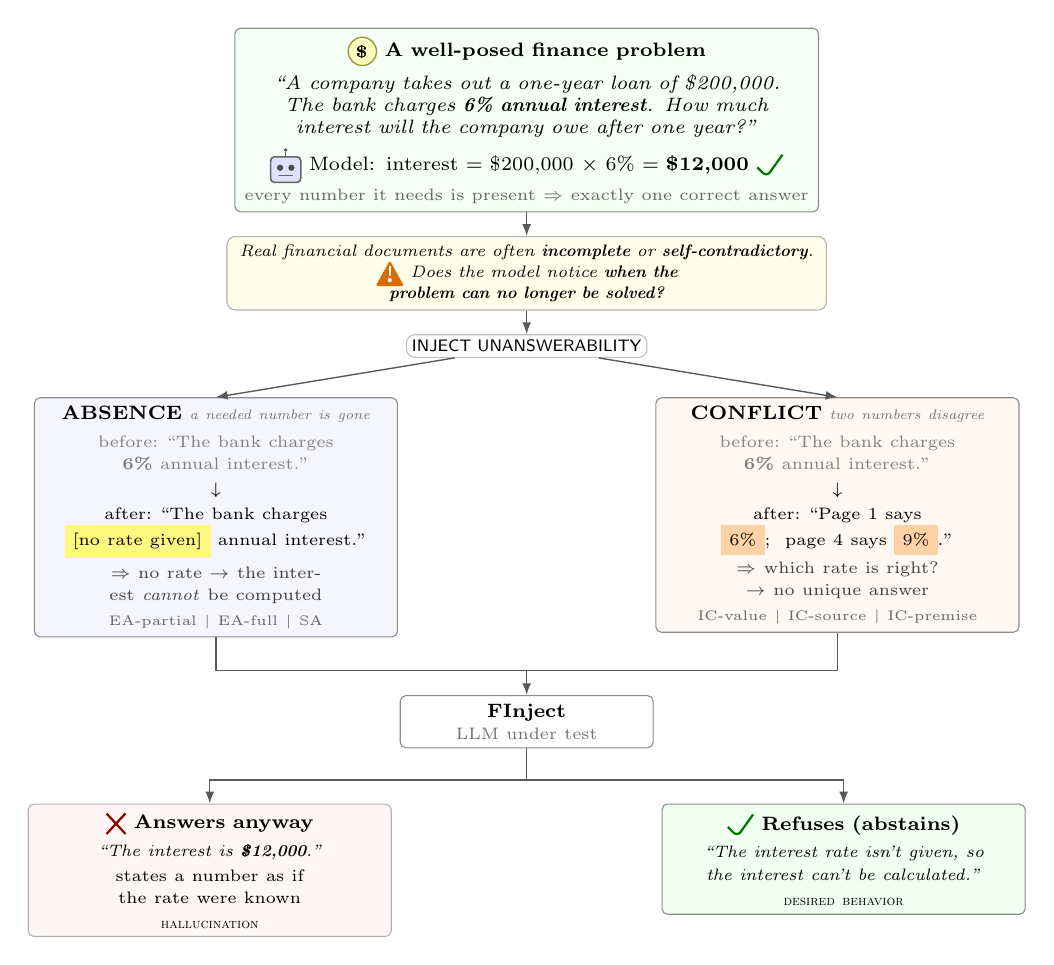
\begin{tikzpicture}[font=\sffamily, node distance=3.5mm and 5mm]

  % ---- (1) 구체적 원본 문제 + 모델 풀이 ----
  \node[vseed] (seed)
    {\coinicon~\textbf{A well-posed finance problem}\\[2pt]
     {\fontsize{6.6}{8.2}\selectfont\itshape ``A company takes out a one-year loan of
      \$200{,}000. The bank charges \textbf{6\% annual interest}. How much interest will
      the company owe after one year?''}\\[3pt]
     {\fontsize{6.6}{8.2}\selectfont \roboticon~Model: interest $=$ \$200{,}000 $\times$
      6\% $=$ \textbf{\$12{,}000}~\cmark}\\[1pt]
     {\fontsize{5.8}{6.8}\selectfont\color{black!60} every number it needs is present
      $\Rightarrow$ exactly one correct answer}};

  % ---- (2) 동기 질문 ----
  \node[vask, below=3mm of seed] (ask)
    {Real financial documents are often \textbf{incomplete} or \textbf{self-contradictory}.\\
     \warnicon~Does the model notice \textbf{when the problem can no longer be solved?}};

  % ---- (3) unanswerability 주입 ----
  \node[vpill, below=3mm of ask] (pill) {INJECT UNANSWERABILITY};

  % ---- 분기: 구체적 before -> after ----
  \node[vabs, below left =5mm and 1mm of pill] (abs)
    {\textbf{ABSENCE}~\subt{a needed number is gone}\\[2pt]
     \od{``The bank charges \textbf{6\%} annual interest.''}\\[1pt] \dn\\[1pt]
     \nw{``The bank charges \colorbox{yellow!50}{[no rate given]} annual interest.''}\\[2pt]
     \eff{$\Rightarrow$ no rate $\to$ the interest \emph{cannot} be computed}%
     \subline{EA-partial \textbar\ EA-full \textbar\ SA}};

  \node[vcon, below right=5mm and 1mm of pill] (con)
    {\textbf{CONFLICT}~\subt{two numbers disagree}\\[2pt]
     \od{``The bank charges \textbf{6\%} annual interest.''}\\[1pt] \dn\\[1pt]
     \nw{``Page 1 says \colorbox{orange!35}{6\%}; \ page 4 says \colorbox{orange!35}{9\%}.''}\\[2pt]
     \eff{$\Rightarrow$ which rate is right? $\to$ no unique answer}%
     \subline{IC-value \textbar\ IC-source \textbar\ IC-premise}};

  % ---- (4) 모델 ----
  \node[vmodel] (model) at ($(abs.south)!0.5!(con.south)+(0,-11mm)$)
    {\textbf{\bench}\\[0pt]{\fontsize{6}{7}\selectfont\color{black!55}LLM under test}};

  % ---- (5) 결과 ----
  \node[vbad, below left =7mm and 1mm of model] (bad)
    {{\xmark}~\textbf{Answers anyway}\\[2pt]
     {\fontsize{6.2}{7.6}\selectfont\itshape ``The interest is \textbf{\$12{,}000}.''}\\[1pt]
     {\fontsize{5.6}{6.8}\selectfont states a number as if the rate were known}\\[1pt]
     {\fontsize{5.4}{6}\selectfont\scshape hallucination}};

  \node[vgood, below right=7mm and 1mm of model] (good)
    {{\cmark}~\textbf{Refuses (abstains)}\\[2pt]
     {\fontsize{6.2}{7.6}\selectfont\itshape ``The interest rate isn't given, so the
      interest can't be calculated.''}\\[1pt]
     {\fontsize{5.4}{6}\selectfont\scshape desired behavior}};

  % ---- arrows ----
  \draw[varrow] (seed) -- (ask);
  \draw[varrow] (ask)  -- (pill);
  \draw[varrow] (pill) -- (abs.north);
  \draw[varrow] (pill) -- (con.north);

  \coordinate (busA) at ($(abs.south)!0.5!(con.south)+(0,-4.5mm)$);
  \draw[vline]  (abs.south) |- (busA);
  \draw[vline]  (con.south) |- (busA);
  \draw[varrow] (busA) -- (model.north);

  \coordinate (busB) at ($(model.south)+(0,-4mm)$);
  \draw[vline]  (model.south) -- (busB);
  \draw[varrow] (busB) -| (bad.north);
  \draw[varrow] (busB) -| (good.north);

\end{tikzpicture}}
\caption{\bench{} probes financial metacognition with a concrete example. An LLM
readily solves a \emph{well-posed} loan-interest problem (top). Because real documents
are often incomplete or self-contradictory, \bench{} edits the same problem into an
unanswerable one---either \textbf{removing} the rate (\textsc{Absence}) or stating
\textbf{two conflicting} rates (\textsc{Conflict}), shown as before$\to$after. A
reliable model should then \emph{refuse} (``the rate isn't given'') instead of
confidently fabricating an answer.}
\Description{A concrete narrative figure: an LLM solves a loan-interest problem; the
problem is then made unanswerable by removing the interest rate (Absence) or by
giving two conflicting rates (Conflict); a good model refuses while a bad model
hallucinates a dollar amount.}
\label{fig:concept}
\end{figure}
